\documentclass{article}
\usepackage{graphicx} % Required for inserting images
\usepackage{minted}
\usepackage{listings}
\usepackage{float}
\usepackage[T1]{fontenc}
\usepackage{titling}
\usepackage{subfig}
\usepackage{url}
\setlength{\droptitle}{-5em}   % This is your set screw
\usepackage[margin=0.5in]{geometry}
\usepackage[backend=biber]{biblatex}
\addbibresource{main.bib}
\title{CSE220 Lab 3 Final Report}
\author{Arjun Vedantham \\ Qingyang Sun}
\date{December 2024}

\begin{document}

\maketitle

\section{Introduction}
We implemented Best Offset Hardware Prefetching, by Pierre Michaud. \cite{7446087}
\subsection{Algorithm overview}
For an incoming cache access for address $X$, we issue a prefetch request for address $X+D$. This offset $D$ is determined by keeping a \textit{recent requests table} and a \textit{score table}. 

For the incoming address $X$, we take a test offset $d_i$, and calculate an address $X - d_i$. If $X - d_i$ is in the recent requests table, we increment the score for offset $d_i$ in the \textit{score table}. We then store the \textit{base address} $X$ in the recent requests table for future lookups. 

In each round, every offset is tested once upon receiving an incoming cache access. At the end of each round (and every offset has been tested once), the offset with the greatest score is chosen as our new offset $D$. 
We then wipe the score table, and restart the learning process. 

In addition, we designate two constants, ROUNDMAX and SCOREMAX. ROUNDMAX denotes the maximum number of rounds before the offset with the greatest score is chosen, and SCOREMAX denotes the maximum
score that an offset can have before it is automatically chosen as the new offset $D$. 

\section{Implementation}
\subsection{Code Organization}
We created and modified several files while implementing this prefetcher. We created a pref\_best\_offset.c source file and a pref\_best\_offset.h header file, based on the 
prefetcher implementations that were already in Scarab. From there, we created a struct type for storing the recent requests table, score table, and offsets. We then modified pref\_table.def, 
which contains pointers to the functions that are used by the cache infrastructure to signal cache hits or misses to the prefetcher module. 

\subsection{Development Challenges}
During development, we ran into a few bugs in our implementation and in Scarab generally. First, we misunderstood the paper initially and believed that offsets should get a penalty upon a miss, which led to incredibly poor cache behavior since scores for offsets could never accumulate. In addition, we were
not calculating the prefetch address correctly. We initially added the offset to the least significant bits of the base address, when we should have been bit shifting the offset to guarantee that we fetch a new cache line. 
One of the most difficult bugs was actually being able to detect prefetch hits. Although the prefetcher table (in pref\_table.def) has a slot for a function pointer that is used when there is an initial hit to a prefetched cache line, the MLC implementation does not actually invoke this function.
We modified the \lstinline{mem_process_mlc_hit_access} function to ensure it was calling the \lstinline{pref_bo_umlc_prefhit} function.

\section{Evaluation}
We evaluated our best offset prefetcher at each layer of the simulated cache hierarchy in Scarab. At each level, we used the size, associativity, line size, and cycle-level latency parameters described in the baseline microarchitecture. These parameters are as follows (in the N/A case, we use the default value in Scarab's Sunny Cove parameters file): 

\begin{center}
        \begin{tabular}{ |c|c|c|c|c|c| } 
        \hline
        Cache level & Size & Associativity & Line size & Cycle latency & Banks \\
        \hline
        DCache & 32KB & 4 & 64 & 3 & 8 \\
        \hline
        MLC & 512KB & 8 & 64 & 11 & N/A \\
        \hline 
        LLC & 8MB & 16 & 64 & 21 & N/A \\ 
        \hline
        \end{tabular}
\end{center}

In addition to these parameters, we also evaluated the architecture without any prefetching enabled, and with the default prefetcher configuration (stream prefetching at the data cache level).

\section{Results}
\subsection{IPC}
\begin{figure}[H]
    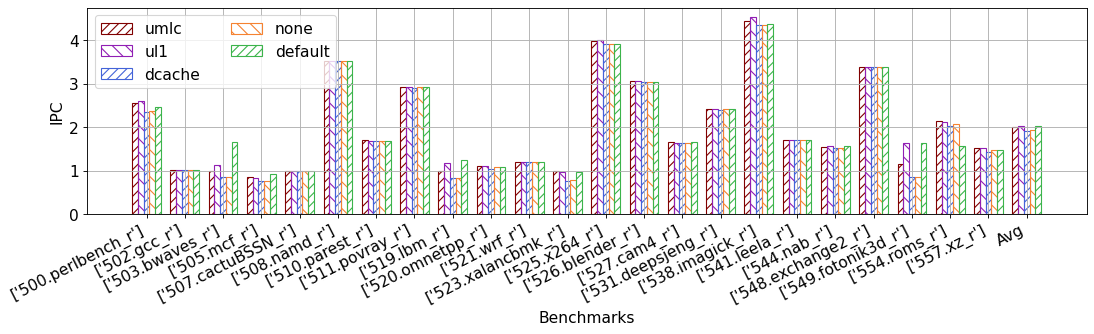
\includegraphics[width=\linewidth]{bo_periodic_PC.png}
\end{figure}
For IPC, we can see that best offset prefetching at the last layer cache and the mid-level cache leads to generally better performance compared to not prefetching at all. For some workloads, the stream prefetcher (operating at dcache) is able to outperform our prefetcher, and prefetching into the last layer cache generally leads to higher IPC compared to prefetching into the mid-level cache.

This may be due to a number of factors. The last layer cache has higher associativity and a larger size overall, thus allowing us to get more hits for a line once it has been prefetched. There may also be a greater variance in the distribution of offsets for a larger cache size (thus allowing us to prefetch lines that are much further away from a current base address), but we were not able to measure the variance of the offset choice, so we cannot confirm this. 
\subsubsection{IPC Speedup}
\begin{figure}[H]%
    \centering
    \subfloat[\centering IPC speedup over no prefetching]{{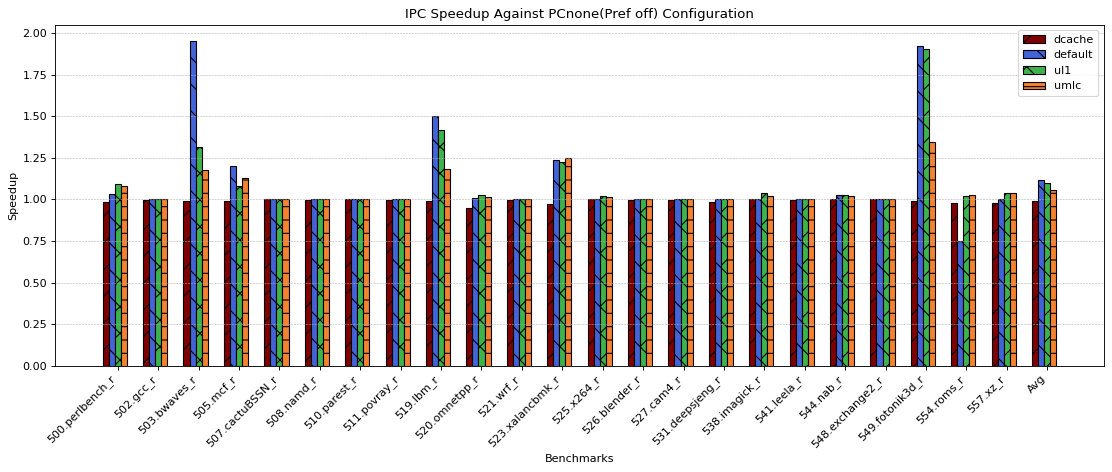
\includegraphics[width=0.45\linewidth]{ipc_speedup_comparison_pcnonePref_off.png} }}%
    \qquad
    \subfloat[\centering IPC speedup over default prefetcher config]{{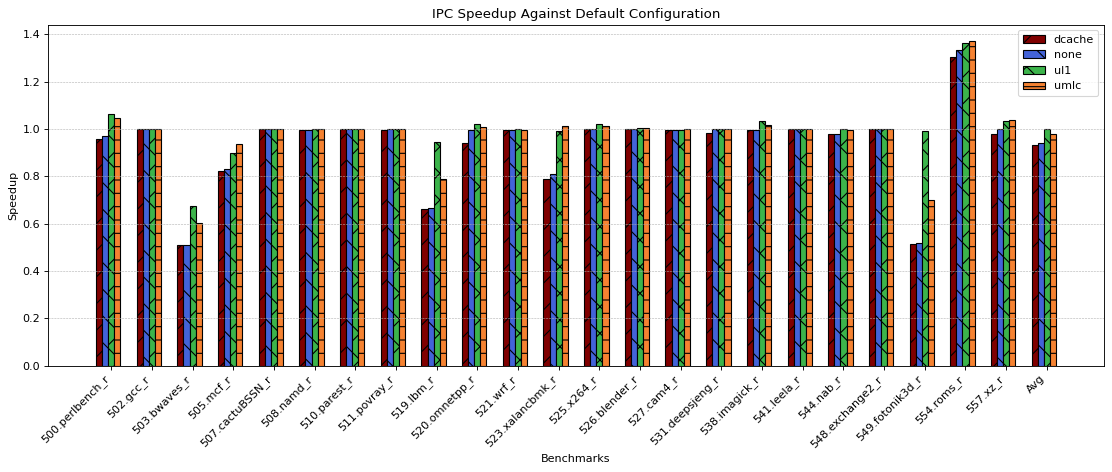
\includegraphics[width=0.45\linewidth]{ipc_speedup_comparison.png} }}%
    \caption{Best offset prefetcher speedup}%
    \label{fig:example}%
\end{figure}
% \begin{figure}[H]
%     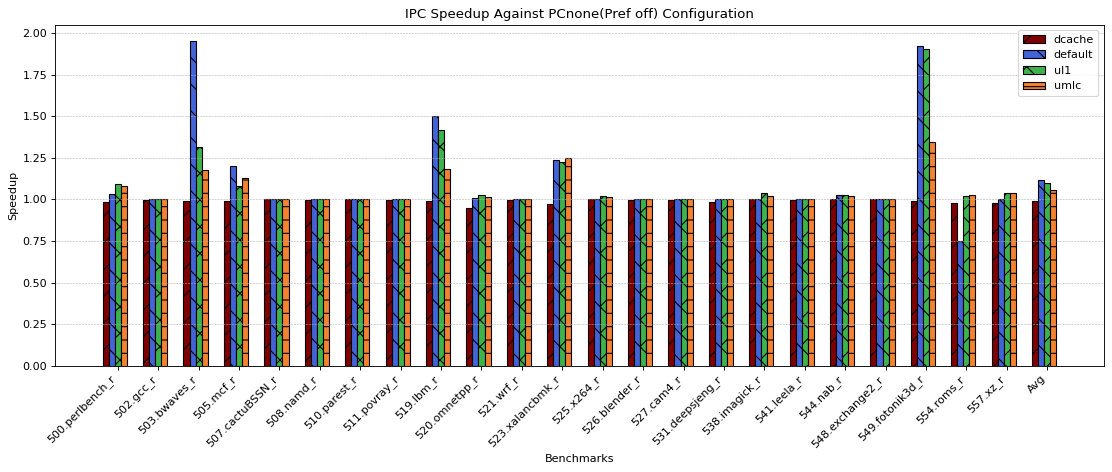
\includegraphics[width=\linewidth]{ipc_speedup_comparison_pcnonePref_off.png}
% \end{figure}
% \begin{figure}[H]
%     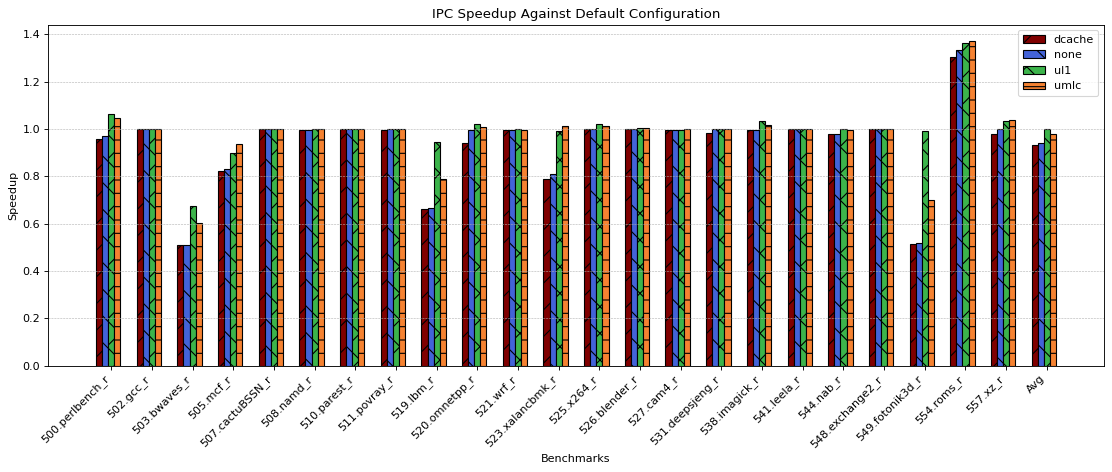
\includegraphics[width=\linewidth]{ipc_speedup_comparison.png}
% \end{figure}
When we evaluate the speedup, we can see that best offset prefetching into the LLC/MLC layers usually outperforms no prefetching, with only prefetching directly into the data cache underperforming. We also outperform the default stream prefetcher relative on some benchmarks, notably the 554 benchmark, where is slows down considerably relative to turning off prefetching entirely.
\subsection{Data Cache Hits vs. Misses}
We also evaluated the number of cache misses at the data cache level. 
\begin{figure}[H]%
    \centering
    \subfloat[\centering Data cache miss rate (\%)]{{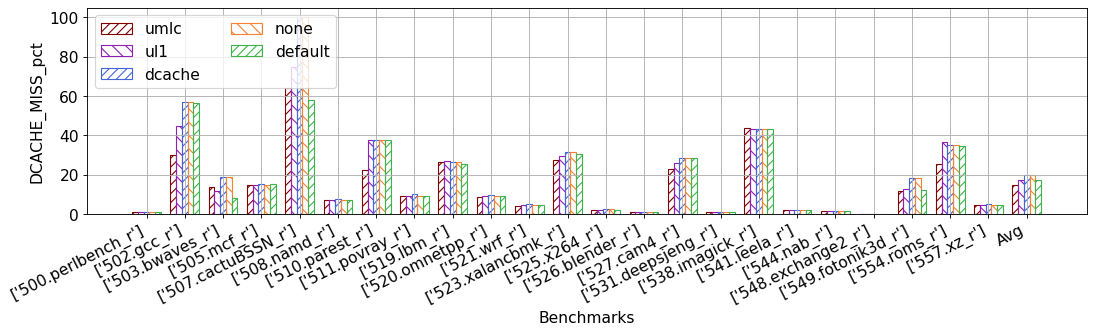
\includegraphics[width=0.45\linewidth]{bo_DCACHE_MISS_pct.png} }}%
    \qquad
    \subfloat[\centering Data cache hit rate (\%)]{{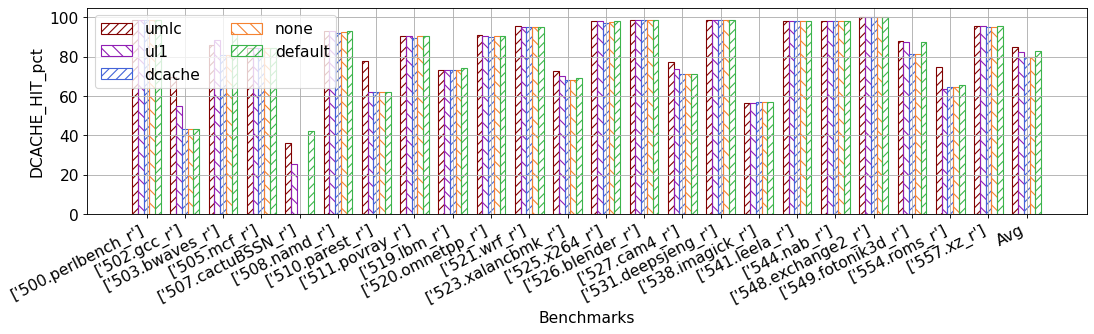
\includegraphics[width=0.45\linewidth]{bo_DCACHE_HIT_pct.png} }}%
    \caption{Miss vs. hit rates at the data cache level for best offset prefetcher}%
    \label{fig:example}%
\end{figure}
In general, prefetching with best offset produced noticeably fewer misses than not prefetching at all, and about on par with the number of cache misses we would see with the default prefetcher configuration. Prefetching into the MLC or LLC was typically better than prefetching into the data cache directly, likely because of the data cache's low size and associativity.
\section{Conclusion}
Altogether, we were able to get our best offset prefetcher working at each layer of the simulated cache hierarchy, and show that it performs evenly, or even better than the default prefetcher for most workloads, and far better than disabling prefetching entirely. If we had more time, we would like to evaluate the distribution of offsets chosen, and profile workloads to better understand the prefetcher's choice of offset. 
The code for our implementation is available on GitHub, at \url{https://github.com/javathunderman/scarab/tree/lab3}.
\printbibliography
\end{document}
